\documentclass[11pt]{article}
\usepackage[margin=1in]{geometry}
\usepackage{graphicx,booktabs,hyperref,float}
\title{Reading Revit (\texttt{.rvt}) Files Without Revit\\\large Test Report}
\author{RNGD side-testing project}
\date{\today}
\begin{document}
\maketitle
\section{Summary}
Three archives were extracted from \texttt{Testt/}, yielding three Revit~2022 sample
models. \textbf{The architecture and structural archives contain the byte-identical file}
(\texttt{racbasicsampleproject.rvt}, same MD5), so only two distinct models exist.
Using only \texttt{olefile} and \texttt{zlib} we can read: file metadata, the embedded
thumbnail, and the element database's text (level, room, family and view names).
We \emph{cannot} recover 3D geometry; that needs Revit, Autodesk Platform Services
or Dynamo. The included tools are a Python module (\texttt{rvt\_tools.py}), a CLI, a
Streamlit viewer, and a 17-test pytest suite (all passing).

\section{Method}
An \texttt{.rvt} is an OLE2 compound file. \texttt{BasicFileInfo} gives the Revit version
and build; \texttt{RevitPreview4.0} holds a PNG thumbnail; \texttt{Partitions/12} is the
element database, stored as many raw-deflate chunks behind gzip headers. Decompressing
every valid chunk and scanning for UTF-16 strings yields names of levels, rooms and
families. Category counts are keyword hit counts, a heuristic and not exact element counts.

\section{Architecture model}
\begin{tabular}{ll}\toprule
File & \texttt{racbasicsampleproject.rvt} \\
Size & 18.61 MB \\
Revit version / build & 2022 / 20210129\_1515(x64) \\
\bottomrule\end{tabular}

\begin{figure}[H]\centering
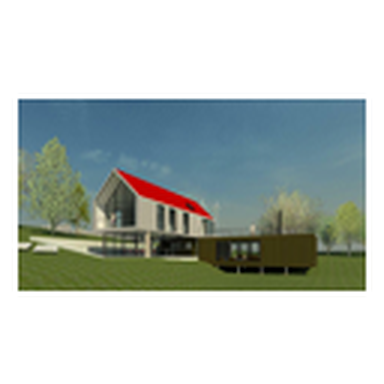
\includegraphics[width=0.45\linewidth]{preview_architecture.png}
\caption{Embedded preview thumbnail (128\,px original, upscaled 3$\times$).}
\end{figure}
\begin{figure}[H]\centering
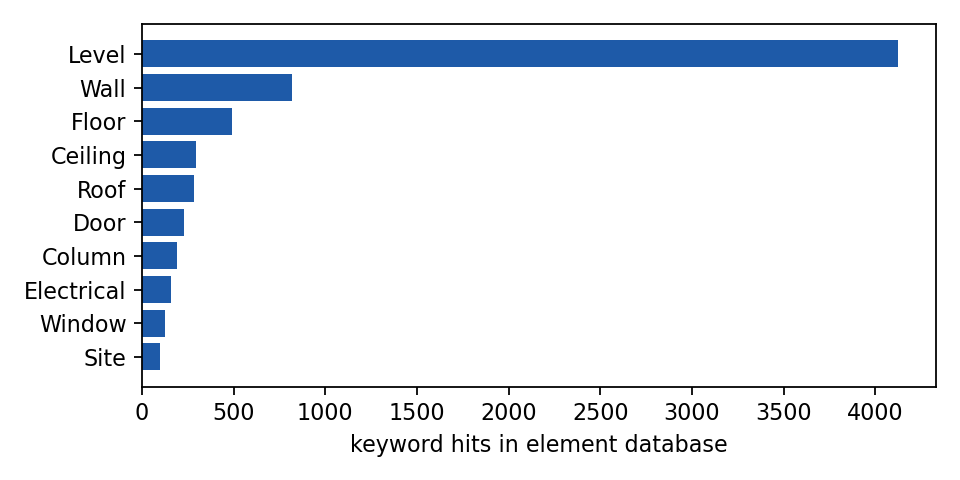
\includegraphics[width=0.8\linewidth]{cats_architecture.png}
\caption{Category keyword signal (heuristic).}
\end{figure}
\noindent Sample recovered names: levels: Level Head - Upgrade, Level 1, Level 2, Floor Plan Level 1;
bedrooms: Bedroom, Master Bedroom, Dormitory Bedroom);
kitchen items: Vault(TM) offset kitchen sink with four-hole faucet drilling, 4500\_Kitchen Island, Kitchen \& Dining.

\section{Mep model}
\begin{tabular}{ll}\toprule
File & \texttt{rmeadvancedsampleproject.rvt} \\
Size & 36.61 MB \\
Revit version / build & 2022 / 20210129\_1515(x64) \\
\bottomrule\end{tabular}

\begin{figure}[H]\centering
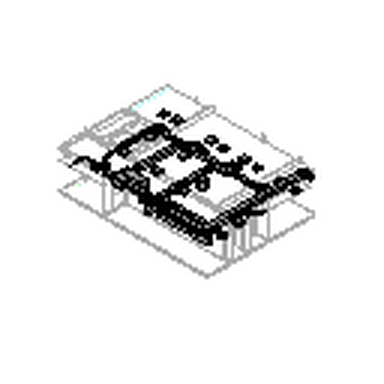
\includegraphics[width=0.45\linewidth]{preview_MEP.png}
\caption{Embedded preview thumbnail (128\,px original, upscaled 3$\times$).}
\end{figure}
\begin{figure}[H]\centering
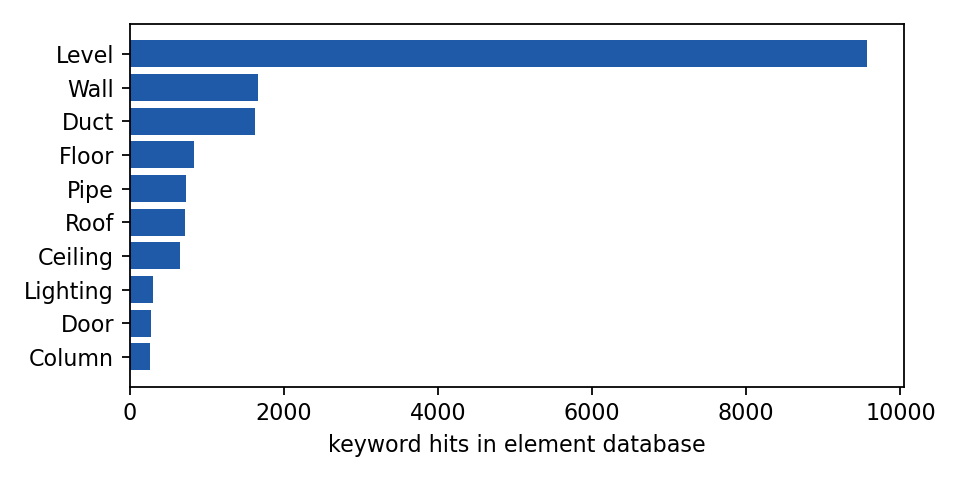
\includegraphics[width=0.8\linewidth]{cats_MEP.png}
\caption{Category keyword signal (heuristic).}
\end{figure}
\noindent Sample recovered names: levels: Level 1, Level Head - Upgrade, Level 2, Level 3;
bedrooms: none;
kitchen items: Sinks - Kitchen.

\section{Structural model}
\begin{tabular}{ll}\toprule
File & \texttt{racbasicsampleproject.rvt} \\
Size & 18.61 MB \\
Revit version / build & 2022 / 20210129\_1515(x64) \\
\bottomrule\end{tabular}

\begin{figure}[H]\centering
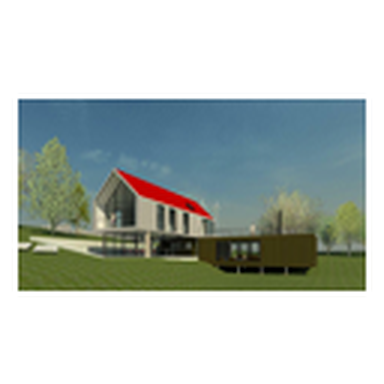
\includegraphics[width=0.45\linewidth]{preview_structural.png}
\caption{Embedded preview thumbnail (128\,px original, upscaled 3$\times$).}
\end{figure}
\begin{figure}[H]\centering
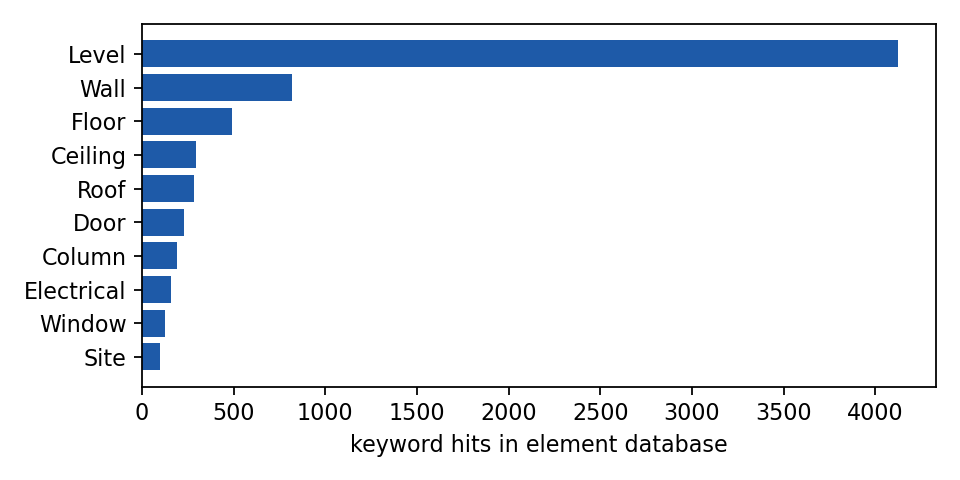
\includegraphics[width=0.8\linewidth]{cats_structural.png}
\caption{Category keyword signal (heuristic).}
\end{figure}
\noindent Sample recovered names: levels: Level Head - Upgrade, Level 1, Level 2, Floor Plan Level 1;
bedrooms: Bedroom, Master Bedroom, Dormitory Bedroom);
kitchen items: Vault(TM) offset kitchen sink with four-hole faucet drilling, 4500\_Kitchen Island, Kitchen \& Dining.

\section{pyRevit integration}
pyRevit v6.5.5.26237 was installed per-user
(\texttt{\%APPDATA\%/pyRevit-Master}). \textbf{Revit itself is not installed on this machine}
(\texttt{pyrevit env} lists no Revit installs), so pyRevit cannot attach and scripts that use the
Revit API cannot run here. Two layers were built:
\begin{enumerate}
\item \textbf{Works now, no Revit:} \texttt{pyrevit\_tools.py} wraps
\texttt{pyrevit revits fileinfo}, which reads project name, client, build, workshared flag and
document GUID directly from the file. Results (identical files de-duplicated):
\end{enumerate}
\begin{center}\small\begin{tabular}{lllll}\toprule
File & Project name & Client & Doc ID & Workshared \\ \midrule
racbasicsampleproject.rvt & Sample House & Autodesk & c26966e9 & No \\
rmeadvancedsampleproject.rvt & Project Name & Owner & 74792680 & No \\
\bottomrule\end{tabular}\end{center}
\begin{enumerate}\setcounter{enumi}{1}
\item \textbf{Needs Revit:} the extension \texttt{pyrevit\_extension/RNGDTest.extension}
(registered in pyRevit's search path) adds an \emph{RNGD} ribbon tab with two buttons:
\emph{Summarize model} (element counts per category, levels, rooms with areas, wall types $\rightarrow$ JSON)
and \emph{Export walls} (centerlines, heights, types $\rightarrow$ JSON). These are \textbf{untested}
until Revit is available; \texttt{pyrevit\_tools.load\_revit\_summary} reads their output.
\end{enumerate}
The RVT sample files were saved by Revit 2022 (build 20210129); opening them needs Revit 2022 or newer.

\section{Limitations and next steps}
\begin{itemize}
\item Only a 128\,px thumbnail is embedded; there is no geometry to render here.
\item For real geometry/quantities: Autodesk Platform Services Model Derivative API
(cloud, needs an APS key), or Revit/Dynamo/pyRevit locally.
\item The string harvest is heuristic; treat category counts as relative signal only.
\item Relevance to RNGD: these sample models could seed the BaaP catalog work once
extraction via APS or Revit is available.
\end{itemize}
\end{document}
